\chapter{Desarrollo}\label{chap:desarrollo}

Este capítulo se centra en explicar cómo se ha llevado a cabo el desarrollo específico de la contribución.
Se empezará por una presentación del escenario real que ha servido de fuente de datos, detallando cómo se han extraído y filtrado los datos.
Una vez vista la manera de reducir el volumen y obtener la información de interés, se expondrán los pasos de análisis y preprocesado previos al \emph{clustering}, así como su parametrización.
Se hará hincapié también en de qué manera se seleccionan las características más importantes para aplicar algoritmos.

\section{Presentación del escenario}\label{sec:presentaciondelescenario}

En el escenario del proyecto (la red de un banco), el tráfico atraviesa distintos equipos de seguridad según el entorno al que corresponda.
Si se trata de tráfico que procede de los usuarios externos conectándose a servicios públicos del banco (expuestos a Internet), se cursa a través de una batería de equipos formada por:
un IPS PaloAlto, un WAF\footnote{\emph{Web Application Firewall}} de marca Fortinet, balanceadores F5, otros firewalls Checkpoint y, finalmente, los servidores.
En caso de ser tráfico desde la red corporativa hacia Internet, los equipos en este camino son el IPS PaloAlto mencionado (pero en esta ocasión está funcionando solo como IDS) y un firewall Fortinet, en este orden.
Si son conexiones internas entre diferentes organizaciones, se procesa con otro firewall Fortinet independiente, etc.

\begin{figure}[h]
    \centering
    \captionsetup{width=12cm}
    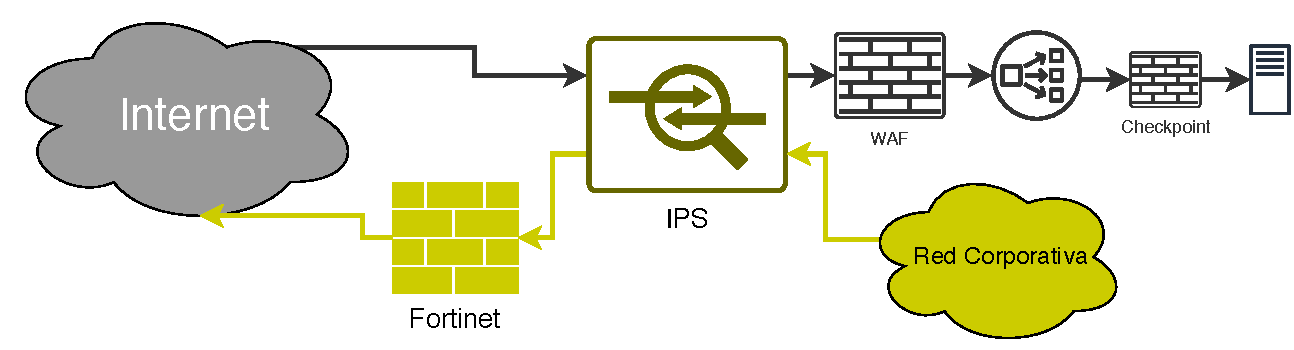
\includegraphics[width=12cm]{contenido/fig/diagrama_red.pdf}
    \caption{Diagrama del tratamiento de conexiones entrantes y salientes}
    \label{fig:diagramared}
\end{figure}

El objetivo de este trabajo se centra en la clasificación de los equipos de la red empresarial, así que se pondrá la atención sobre el segundo itinerario descrito, de color amarillo en la figura \ref{fig:diagramared}: el tráfico saliente, desde la red hacia Internet.
En especial, se quiere exprimir la información que proporciona el firewall Fortinet de ``Internet Corporativo'', ya que es principalmente quien reacciona con mecanismos de prevención o bloqueos ante las acciones iniciadas en la red corporativa.
Como se ha explicado, al estar el IPS actuando como IDS en este ámbito y además procesando tráfico de otras redes y en otras direcciones, su información nos interesa menos.
Sin embargo, si en un momento dado del desarrollo de este método de \emph{clustering} se cree beneficioso incorporar los eventos que arroja el IPS sobre las sesiones de los hosts de la red,
será necesario que se hayan analizado correctamente y puedan extraerse con facilidad.
Por eso, en la siguiente sección se detalla cómo se han estudiado los logs de ambos.

\section{Extracción y filtrado}\label{sec:extraccionyfiltrado}

El punto de interés para la captura se concentra por tanto en dos equipos por los que pasa el grueso del tráfico total: un firewall Fortinet y un IPS PaloAlto.
Como es habitual, estos equipos reportan todas sus acciones a través de logs, con varios niveles de granularidad e importancia.
Incluyen también multitud de información aportada por los propios sistemas que enriquecen el valor de cada evento.
Esto es razón para preferir los logs de firewall como fuente de información frente a una captura de tráfico en crudo, ya que
lo que procesan los firewalls casi siempre es más relevante que el tráfico completo pero sin procesar.
Además, el volumen de una captura de tráfico sería notablemente mayor y más difícil de manejar.

La cantidad de datos recibida en los logs sigue siendo alta, pero además necesita ser procesada para obtener datos útiles.
En los párrafos siguientes se explica cómo se han extraído los datos de sesión que se usarán como materia prima para tener finalmente unos datos de entrada al algoritmo de \emph{clustering}.
Se ha tomado una semana de muestra para trabajar con un periodo acotado.
Nótese en la figura \ref{fig:volumenlogs} la reducción en esta primera etapa del volumen de los datos, que seguirán transformándose en sucesivas fases hasta mantener únicamente la información valiosa para la tarea que nos ocupa.

\begin{figure}[h]
    \centering
    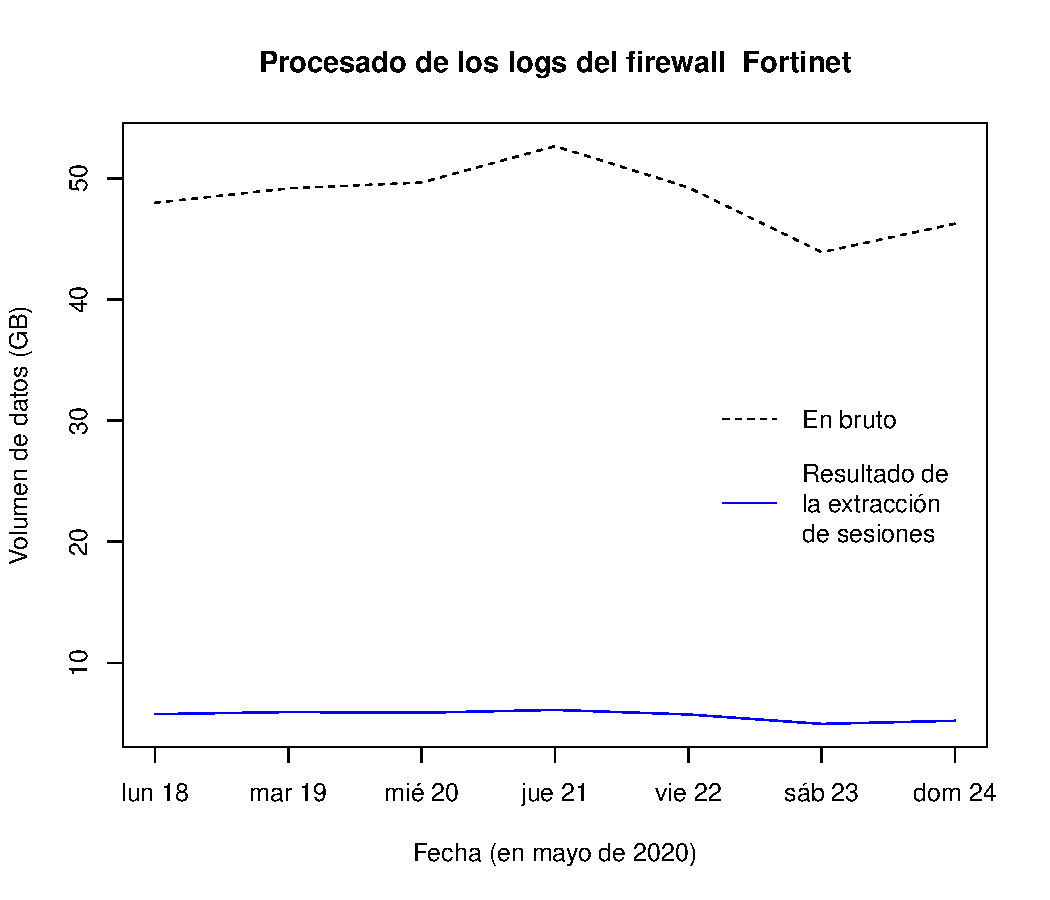
\includegraphics[width=0.55\textwidth]{contenido/fig/volumen_logs.pdf}
    \caption{Volumen de logs en bruto y tras ser procesados, en una semana}
    \label{fig:volumenlogs}
\end{figure}

Aunque el fin para el que sirven ambos equipos (análisis y protección frente a amenazas informáticas) sea similar,
la estructura usada por cada uno en los logs que produce es completamente distinta.
Los logs de Fortinet siguen un formato clave-valor con ciertas particularidades, mientras que los de PaloAlto tienen una serie de campos fijos que están delimitados por comas.
A modo de ejemplo, las dos líneas adjuntadas a continuación corresponden a un evento del firewall Fortinet y otro del IPS PaloAlto, respectivamente (viene un evento por línea):

\begingroup
\makeatletter
\@totalleftmargin=-1cm
\begin{verbatim}

1585572524|1585572524|2020-03-30T06:48:44.202297|10.2.0.11|6|local7|
date=2020-03-30 time=06:48:44 devname="FW1_INTERNETCORP" devid="FG1809999"
logid="1059028704" type="utm" subtype="app-ctrl" eventtype="app-ctrl-all"
level="information" vd="root" eventtime=1585572524 appid=41470 user="NOM"
group="GrupoOffice365" authserver="SV1" srcip=172.2.9.6 dstip=23.203.51.72
srcport=54697 dstport=443 srcintf="p18" srcintfrole="undef" dstintf="p20"
dstintfrole="wan" proto=6 service="HTTPS" direction="outgoing" policyid=124
sessionid=325186437 applist="AC_CORREO" appcat="Collab" app="Microsoft.CDN"
action="pass" hostname="img-prod-cms-rt-microsoft-com.akamaized.net"
incidentserialno=1513678724 url="/" msg="Collaboration: Microsoft.CDN,"
apprisk="elevated" scertcname="a248.e.akamai.net"

1585659863|1585659863|2020-03-31T07:04:23.027791|10.2.0.73|6|local0|
1,2020/03/31 07:04:23,001801037558,TRAFFIC,end,2049,2020/03/31 07:04:03,
10.138.4.7,186.151.236.155,0.0.0.0,0.0.0.0,OUTBOUND,,,incomplete,vsys1,
trust,untrust,ethernet1/10,ethernet1/9,Log-Panorama,2020/03/31 07:04:03,
41602,1,55074,80,0,0,0x19,tcp,allow,132,132,0,2,2020/03/31 07:03:55,3,any,
0,1307298109,0x80000,10.0.0.0-10.255.255.255,America,0,2,0,aged-out

\end{verbatim}
\endgroup

Otro hecho reseñable que afecta al formato es que se emplea \emph{syslog} \cite{RFC5424} (el estándar de facto)
como protocolo para trasladar los datos desde cada equipo hasta el punto de recolección,
de forma que se cuenta con ciertos campos adicionales a los enviados por los equipos.
Para el tema que nos ocupa, los únicos campos que se extraen de esta cabecera son:
la marca de tiempo en la que ha llegado cada evento, conocida en el vocabulario informático como \emph{timestamp}, y lo que conoceremos como la prioridad del evento
(que en la especificación de \emph{syslog} se denomina severidad, pero se ha creído que el término ``prioridad'' es más acertado en este entorno).
En cualquier caso, esta sección adicional dentro de los logs tiene también su propio formato, por lo cual también se deberá tratar de forma específica.
En nuestra configuración (que aplica a la herramienta \emph{rsyslog}\footnote{\url{https://www.rsyslog.com/}}),
la siguiente directiva establece cómo se vuelcan a fichero estos campos de syslog:

\begin{verbatim}
template(name="FORMATO_LOGS" type="string"
string="%timereported:::date-unixtimestamp%
    |%timegenerated:::date-unixtimestamp%
    |%timegenerated:::date-rfc3339%|%fromhost-ip%
    |%syslogseverity%|%syslogfacility-text%| %syslogtag%%msg%\n")
\end{verbatim}

Así que, en los \emph{scripts} que procesan los ficheros donde se han volcado los datos traídos mediante \emph{syslog},
se obtiene la fecha de cada evento a partir de este primer campo ``timereported:::date-unixtimestamp'' y la prioridad a partir del quinto campo.
Esta primera parte del procesado (que está programado en Python) se hace de la siguiente manera:

\begin{minted}{python}
for syslogline in sys.stdin:

    try:

        splitted_syslogline = syslogline.rstrip().split("|") # .rstrip() removes last "\n" character

        tstamp_line = int(splitted_syslogline[0])

        prio = splitted_syslogline[4]
\end{minted}

Seguidamente, el resto de la línea actual (sin la cabecera de \emph{syslog}) se convierte en una estructura de diccionario.
Como se apreciaba en las líneas de ejemplo que se han incluido antes, la relación entre claves y valores depende de cada caso.

Para el equipo Fortinet, la relación está definida en el propio evento como \texttt{clave="valor"} o \texttt{clave=valor} para valores no considerados como cadenas de texto.
Cabe destacar que el símbolo ``\texttt{=}'' puede estar contenido en el valor.
El nombre de la clave, sin embargo, nunca llevará comillas.
Establecidas las anteriores reglas, en Fortinet se convierten los campos con una expresión regular y una \emph{dict comprehension}\footnote{\url{https://www.python.org/dev/peps/pep-0274/}}
(es decir, una forma concisa de crear diccionarios a través de la iteración sobre una lista con la posibilidad de incluir condicionales):

\begin{minted}{python}
    line = "".join(splitted_syslogline[6:]) # removes "1581410810|1581410810|2020-02-11T02:46:51.421302|10.25.0.6|5|local7|"

    fields = re.split("([^ \"]+=[^ \"]+)|([^ \"]+=\"[^\"]+\")", line)

    dict_line = {k:v.strip('"')
                 for k,v in [f.split("=", 1)
                 for f in fields if (f and "=" in f)]}
\end{minted}

Para el IPS PaloAlto, la extracción de los campos es más sencilla.
Como cumplen con el formato CSV estandarizado \cite{RFC4180}, los valores se tienen en una lista
con solo leer la línea a través de una función de la librería \texttt{csv}.
En cuanto a las claves, en la documentación\footnote{\url{https://docs.paloaltonetworks.com/pan-os/8-1/pan-os-admin/monitoring/use-syslog-for-monitoring/syslog-field-descriptions.html}}
de PaloAlto se explica que depende del tipo del evento.
Por tanto, se asignan unas claves u otras consultando primero de qué tipo se trata.
Finalmente, se construye el diccionario con otra \emph{dict comprehension}:

\begin{minted}{python}
    line = "".join(splitted_syslogline[6:]) # removes "1581410810|1581410810|2020-02-11T02:46:51.421302|10.25.0.6|5|local7|"

    values = list( csv.reader([line]) )[0]

    this_type_keys = []

    if values[3]=="TRAFFIC": # type is on 4th field
        this_type_keys.extend(common_trafficthreat_fields)
        this_type_keys.extend(traffic_fields)
    elif values[3]=="THREAT":
        ...

    if this_type_keys!=[]:
        dict_line = {k:v for k,v in zip(this_type_keys,values)}
\end{minted}

Posteriormente se lleva a cabo otra serie de operaciones necesarias para la transformación de los datos de entrada en información útil para la monitorización.
Sin embargo, desde la perspectiva de este trabajo, el único apartado de interés es la agregación de sesiones, que se desarrolla a continuación.

Una parte de este procesado consiste en guardar cierta información asociada a cada sesión.
El concepto de ``sesión'' sería equivalente al de ``flujo'' presentado en el \hyperref[chap:estadodelarte]{capítulo anterior}:
una serie de eventos asociados que se corresponden con la misma tupla de \{IP origen, IP destino, protocolo, puerto origen, puerto destino\}.
Los dos equipos mantienen un campo ``Identificador de Sesión'' interno que se añade a la tupla de la sesión.
Este campo permite distinguir los eventos de sesiones que coinciden en origen y destino pero se producen en intervalos temporales diferentes.
Se incluye en el procesado con esta finalidad de no confundir sesiones distintas en etapas posteriores, pero para nuestro propósito de clasificación de equipos puede ignorarse.

La información de cada sesión se compone de:
\begin{itemize}
    \item Tupla que define la sesión:\\\{ID de sesión, IP origen, IP destino, protocolo, puerto origen, puerto destino\}
    \item Timestamps del primer y último evento pertenecientes a esta sesión
    \item Máxima prioridad de evento vista en esta sesión
    \item Bytes recibidos y enviados (solo en el IPS)
    \item Nivel de anomalía
    \item Nivel de amenaza
    \item Contador y lista de eventos
\end{itemize}

Los niveles de anomalía y amenaza son unos índices simples que se han diseñado para resumir cualidades de interés acerca de la sesión, como son
cuánto se aleja de la normalidad la cantidad de eventos prioritarios que se han visto y cómo son de peligrosas las amenazas recibidas.
Se entiende como ``evento'' una entrada de log, que está relacionada con una sesión concreta.
Puede comprobarse cómo es un evento en las líneas de logs del firewall Fortinet y del IPS PaloAlto que aparecían como ejemplos al principio de \hyperref[sec:extraccionyfiltrado]{esta misma sección}.

Para cada sesión, se calculan sus niveles sumando los \(n\) eventos que le corresponden, según las siguientes fórmulas:

\begin{eqnarray*}
    & \mathlarger{\mathlarger{\mathlarger{N}}}_{\textrm{anomalía}} = \mathlarger{\mathlarger{\mathlarger{\sum}}}_{i=1}^{n} \frac{1}{\textrm{prioridad}_{\textrm{evento}_i}}\\
    & \textrm{para eventos de prioridad }\leq4\textrm{ o eventos de tráfico que no son de inicio ni fin}
\end{eqnarray*}

\begin{eqnarray*}
    & \mathlarger{\mathlarger{\mathlarger{N}}}_{\textrm{amenaza}} = \mathlarger{\mathlarger{\mathlarger{\sum}}}_{i=1}^{n} \frac{1}{\textrm{prioridad}_{\textrm{evento}_i}}\\
    & \textrm{para eventos de amenaza con prioridad }\leq4\textrm{ que no son bloqueados}
\end{eqnarray*}

Tanto estas como el resto de características cuantificables pueden resultar de interés a la hora de aplicar \emph{clustering} sobre un \emph{dataset} derivado de este procesado.

La recolección de esta información se realiza a través de la función adjunta.
Como puede verse, cuando se llama a esta función (lo cual ocurre ante todos los eventos de protocolo TCP o UDP)
se actualizan los parámetros relativos a la sesión actual, que están almacenados en un diccionario.
A su vez, este diccionario se encuentra dentro del diccionario \texttt{sessions}.
Con él se mantienen en memoria todas las sesiones que todavía no se han cerrado.
Cuando transcurre un \emph{bucket} de tiempo determinado (por defecto, 60 segundos), se comprueban todas las sesiones vigentes.
Aquellas que tienen un evento de finalización se imprimen en un fichero y se retiran del diccionario \texttt{sessions}.
De este modo, cada 60 segundos se tienen los datos de nuevas sesiones completadas (en la práctica se alcanzan incluso más de 100 000 sesiones finalizadas cada minuto).

Esta serie de datos por sesión que produce la función \texttt{session\_aggregation} se denominará ``vector de características de la sesión'', y el conjunto de estos vectores será el contenido en bruto a partir del cual se formará la entrada para el \emph{clustering}.

\begin{minted}{python}
def session_aggregation(dict_line, event_descript, event_tstamp):
    """
    It groups info related to actual session on the sessions dictionary, that is:
    - the sessionid and the session tuple (srcip-dstip-proto-srcport-dstport)
    - tstamp of first and last event observed for actual session
    - update max. priority of events observed for actual session
    - sent and received bytes for actual session
    - counter and list of events observed for actual session
    - recalculate anomaly level for actual session
    - recalculate threat level for actual session
    """

    session_tuple = "···".join([
            dict_line['SESSION ID'], dict_line['SRC_IP'], dict_line['DST_IP'],
            dict_line['PROTO'], dict_line['SRC_PORT'], dict_line['DST_PORT']
        ])

    priority = int(dict_line['priority'])

    if session_tuple not in sessions:
        sessions[session_tuple] = {}
        # store the session tuple values related to this new session_tuple:

        sessions[session_tuple]['events'] = []
        sessions[session_tuple]['anomaly_level'] = 0
        sessions[session_tuple]['threat_level'] = 0
        sessions[session_tuple]["counter"] = 0
        sessions[session_tuple]['max_prio'] = priority
        sessions[session_tuple]["bytes_sent"] = 0
        sessions[session_tuple]["bytes_rcvd"] = 0
        sessions[session_tuple]['first_event_tstamp'] = int(event_tstamp)

    sessions[session_tuple]['last_event_tstamp'] = int(event_tstamp)
    sessions[session_tuple]["counter"] += 1

    if dict_line['type']=="TRAFFIC":
        sessions[session_tuple]["bytes_sent"] += int(dict_line['BYTES_SENT'])
        sessions[session_tuple]["bytes_rcvd"] += int(dict_line['BYTES_RECEIVED'])

    if priority < sessions[session_tuple]['max_prio']:
    # lower prio value means more important (i.e., the most important priority is 1, or even 0 if priority=0 exists)
        sessions[session_tuple]['max_prio'] = priority
    else:
        sessions[session_tuple]['max_prio']

    if priority<=4 or (dict_line['type']=="TRAFFIC" and "end" not in event_descript and "start" not in event_descript):
        sessions[session_tuple]['anomaly_level'] += 1/priority
    if priority<=4 and dict_line['type']=="THREAT" and dict_line['ACTION']!="alert":
        sessions[session_tuple]['threat_level'] += 1/priority

    sessions[session_tuple]['events'].append("{}, {}".format(event_descript, dict_line['ACTION']))
\end{minted}

\section{Preprocesado para el clustering}\label{sec:preprocesado}

A partir de los vectores de características de sesión descritos anteriormente, se debe obtener un \emph{dataset} en el formato adecuado para poder aplicar algoritmos de \emph{clustering} sobre él.
Esta adecuación consistirá básicamente en resumir la información aplicando agregaciones y calculando métricas.

Ya se ha señalado que el volumen de datos es muy alto, así que como primera aproximación se extraerá una muestra suficientemente grande pero operable a priori.
También se empezará por los datos de sesiones vistas en el Fortinet, ya que, al ser el equipo que vigila las conexiones desde la red corporativa a Internet,
resulta de más interés y presumiblemente tendrá una actividad más relevante de cara a clasificarla.

La cantidad de sesiones diaria en el firewall Fortinet suele estar en torno a los 20 millones.
Se practica un muestreo aleatorio simple que reduce los datos a un 5\%,
de forma que el tamaño de la muestra (1 millón de sesiones) sea significativo para obtener unas primeras conclusiones pero su tratamiento no sea excesivamente costoso.

Los datos se guardan en un fichero por día, rotándose a diario y conservándose así (en texto plano, dispuestos para ser importados a una base de datos) durante 14 días antes de eliminarse.
Mediante el siguiente comando, se copian 1 millón de vectores de características de sesión aleatorios, que están formados por:

\{tstamp inicio, tstamp fin, IP origen, IP destino, protocolo, puerto origen, puerto destino, nivel de anomalía, nivel de amenaza, máxima prioridad, cantidad de eventos\}

El comando se repite para los 7 ficheros de una semana:

\begin{verbatim}
$ shuf -n 1000000 FORTINET_INTERNET_CORP_10.251.0.101.1 | \
    awk -F"···" '{print $1,$2,$5,$6,$7,$8,$9,$10,$11,$12,$13,$1-$2}' \
    > datasets_clustering/FORTINET_INTERNET_CORP_10.251.0.101.23may
\end{verbatim}

Y los vectores de características de sesión se vuelcan ordenados por \emph{timestamp} de inicio en un mismo fichero, que es como se leerán para contar cuántas sesiones hay en cada fracción del día:

\begin{verbatim}
$ sort -n datasets_clustering/* > datasets_clustering/rawdata_7days
\end{verbatim}

En las pruebas iniciales se descartaron las marcas de tiempo (campos \verb|$1,$2|) por simplicidad, sabiendo que así se empezaría a trabajar con características más acotadas.
Cuando ya se había validado el flujo de trabajo para aplicar los algoritmos con una cantidad limitada de características y se había adquirido práctica, se incorporaron las variables temporales.
El campo \verb|$1| es el \emph{timestamp} de inicio de sesión, \verb|$2| es el \emph{timestamp} de fin de sesión, y con \verb|$1-$2| se halla la duración de la misma (se incluye por comodidad para cálculos posteriores).
La manera en la que se expresarían como características para el \emph{clustering} requiere ser explicada con más profundidad en los párrafos sucesivos,
donde se desarrollará cómo se han calculado los valores, cómo se ha realizado la agregación y por qué se ha escogido usar estas métricas.

El siguiente paso consiste en agrupar los vectores de características de sesión por IP de origen, que será la característica identificativa de cada \emph{datapoint}.
Para cada valor de la variable ``IP de origen'', se contabilizan cuántos valores distintos se observan en el resto de variables.
Hay ciertas variables que no tiene sentido resumir mediante un recuento, como son: los protocolos usados, los niveles de amenaza y anomalía, la prioridad máxima y las características temporales.

A continuación se detallará lo que significa cada una de las 13 variables finales o características que se han usado.
En la tabla \ref{tab:metricas}, después de los siguientes párrafos de detalles, se sintetiza toda esta información.

Las cuatro primeras características cuentan el número de IPs destino, protocolos, puertos origen y puertos destino que corresponden a una IP origen.
Para distinguir si, en caso de usarse un solo protocolo de nivel de transporte, este es TCP o UDP, el número de protocolos se codifica como se indica:
el valor de ``protocolos usados'' será ``2'' si la IP origen tiene sesiones tanto TCP como UDP, ``1'' si solo emplea UDP, y ``0'' si todas las sesiones son TCP.

Las dos características siguientes, que son los niveles medios de anomalía y amenaza, se hallan calculando la media de cada nivel en todo el periodo de tiempo bajo análisis (un día).

La característica ``prioridad máxima'' corresponde al valor de prioridad más bajo de un evento visto para esta IP origen.
Nótese que los niveles de proridad en \emph{syslog} (más precisamente, lo que \emph{syslog} llama ``severidad'') son descendentes,
siendo 0 el nivel de emergencia, 1 el nivel de alerta, 2 el nivel crítico, 3 error, 4 peligro, 5 aviso, 6 información y por último, como menos importante, 7 depuración.
Por tanto, respetando la definición original de estos niveles de prioridad de los eventos,
se debe tomar como prioridad de máxima importancia aquella prioridad de evento mínima de todas las vistas con esta IP origen.

La característica \texttt{count\_events} es la suma de eventos que el firewall ha asociado a una misma IP origen.

Las últimas cinco características son las relativas al tiempo.

Primero se tienen dos métricas derivadas de la duración de las sesiones:
``media de la duración de sesión'' recoge cuántos segundos han durado de media las sesiones que ha mantenido una IP origen en el día en cuestión,
mientras que ``desviación estándar de la duración de sesión'' cuantifica la variación de la duración de las sesiones respecto de su media.
Con ellas se quiere caracterizar si un equipo (que corresponde a una IP origen) acostumbra a tener sesiones largas o cortas,
y si esas duraciones son habituales o suelen variar mucho.

Las tres variables que cierran el conjunto de características son ``número de sesiones activas en horas nocturnas / horas de trabajo / horas después del trabajo''.
En base a la hipótesis de que será relevante para la clasificación saber en qué momento del día se concentran las sesiones de un equipo,
se ha definido una manera de contabilizar cuántas sesiones mantuvo activas una IP origen en cada fracción del día
(se trabaja con 3 fracciones: horas nocturas de 00:00 a 08:00, horas laborales de 08:01 a 16:00 y horas después del trabajo de 16:01 a 23:59).
Partiendo de todos los vectores de características de sesión ordenados cronológicamente por hora de inicio,
para cada IP origen se incrementa el contador de cada fracción en la que una sesión haya permanecido activa
(esta muestra se divide en $3\textsf{ fracciones/día} \times 7\textsf{ días} = 21\textsf{ fracciones}$).

Las líneas de código que con las que se realiza este conteo son las siguientes:

\begin{minted}{python}
week_tstamps = [i for i in range(1589752800,             1590357601, 60*60*8)]
                              #^^ L18may00:00; so L25may00:00 is included ^^; 8h step^^

slots = ['night', 'work', 'afterwork']
        # 00:00 - 08:00 - 16:00 - 00:00

t=0 # counter of actual element on week_tstamps

for line in raw_data:

    r = line.split()
    initial_tstamp = int(r[0])
    end_tstamp = int(r[1])
    src_ip = r[2]

    if initial_tstamp > week_tstamps[-1]:
    # so all week_tstamps have been covered:
        break

    if initial_tstamp > week_tstamps[t]:
    # so we move forward to the next week fraction:
        t+=1

    data[src_ip]['slots'][slots[ t%len(slots)-1 ]] += 1
    #example:
    # src_ip:10.212.138.53,from 1589807186(15:06:26) to 1589807191(15:06:31)
    #   -> {'night': 0, 'work': 1, 'afterwork': 0}
    # src_ip:10.212.138.53,from 1589920495(22:34:55) to 1589920504(22:35:04)
    #   -> {'night': 0, 'work': 1, 'afterwork': 1}

    i=t
    while end_tstamp > week_tstamps[i]:
    # long sessions count on every slots they are:
        data[src_ip]['slots'][slots[ i%len(slots)-1 ]] += 1
        i+=1
        if i==len(week_tstamps):
        # so end of the observed week has been reached:
            break
\end{minted}

Como resultado de esta transformación (el código completo se adjunta en el apéndice \ref{app:preprocesado}), se tiene una matriz con 13 columnas y \emph{n} filas, siendo \emph{n} el número de IPs de origen distintas presentes en la muestra de ese día.
Cada valor de esta matriz resume las sesiones que un host (identificado por su IP de origen) ha mantenido, a través de las siguientes características o métricas calculadas sobre periodos de un día:

\begin{table}[h]
    \centering
    \begingroup
    \setlength{\tabcolsep}{10pt} % Default value: 6pt
    \renewcommand{\arraystretch}{1.5} % Default value: 1
    \hspace*{-2cm}
    \begin{tabular}{|c|c|}
        \hline
        \textbf{Característica} & \textbf{Explicación} \\
        \hline
        \hline
        Número de IPs destino únicas  & IPs distintas a las que se ha conectado una IP origen \\
        \hline
        Protocolos usados & 2 si IP origen ha usado TCP y UDP, 1 si UDP, 0 si TCP \\
        \hline
        Número de puertos origen únicos & Puertos de nivel transporte usados por una IP origen \\
        \hline
        Número de puertos destino únicos & Puertos a los que se ha conectado una IP origen \\
        \hline
        Nivel de anomalía medio & Media de $N_{\textrm{anomalía}}$ en las sesiones de una IP origen \\
        \hline
        Nivel de amenaza medio & Media de $N_{\textrm{amenaza}}$ en las sesiones de una IP origen \\
        \hline
        Prioridad máxima & Prioridad más crítica vista en eventos de una IP origen \\
        \hline
        Número de eventos & Suma total de los eventos de una IP origen \\
        \hline
        Media de la duración de sesión & Duración media de las sesiones de una IP origen \\
        \hline
        Desv. estándar de la duración de sesión & Desv. est. de la duración de sesiones de una IP origen \\
        \hline
        Nº sesiones activas en horas nocturnas & Sesiones activas de 00:00 a 08:00 \\
        \hline
        Nº sesiones activas en horas de trabajo & Sesiones activas de 08:01 a 16:00 \\
        \hline
        Nº ses. activas en horas después del trabajo & Sesiones activas de 16:01 a 23:59 \\
        \hline
    \end{tabular}
    \hspace*{-1cm}
    \endgroup
    \caption{Características con las que se resumen las sesiones en matrices diarias}
    \label{tab:metricas}
\end{table}

Procediendo análogamente sobre los datos de cada día, obtenidos entre el lunes 25 de mayo de 2020 y el domingo 31,
se tienen 7 matrices de 13 variables por unas 4800 filas (equivalentes al total de IPs origen distintas cada día),
apreciándose un descenso de la cantidad de orígenes únicos en torno al fin de semana
(4700 filas distintas el viernes y alrededor de 3000 filas tanto sábado como domingo).
En total, se dispone de prácticamente 30 000 muestras.
Con este material se puede abordar el prototipado del método de \emph{clustering} sobre el que se fundamenta este proyecto.

\section{Análisis de datos}\label{sec:analisisdedatos}

Una vez obtenidas las características, se pasa a analizar la distribución de valores que presenta cada una de ellas en este \emph{dataset}.
Dicha tarea permitirá entender mejor la importancia relativa de cada característica y cómo afectará a los algoritmos de \emph{clustering}.
En concreto, se prestará especial atención a la forma, varianza y modalidades de las distribuciones.

\begin{figure}[h]
    \centering
    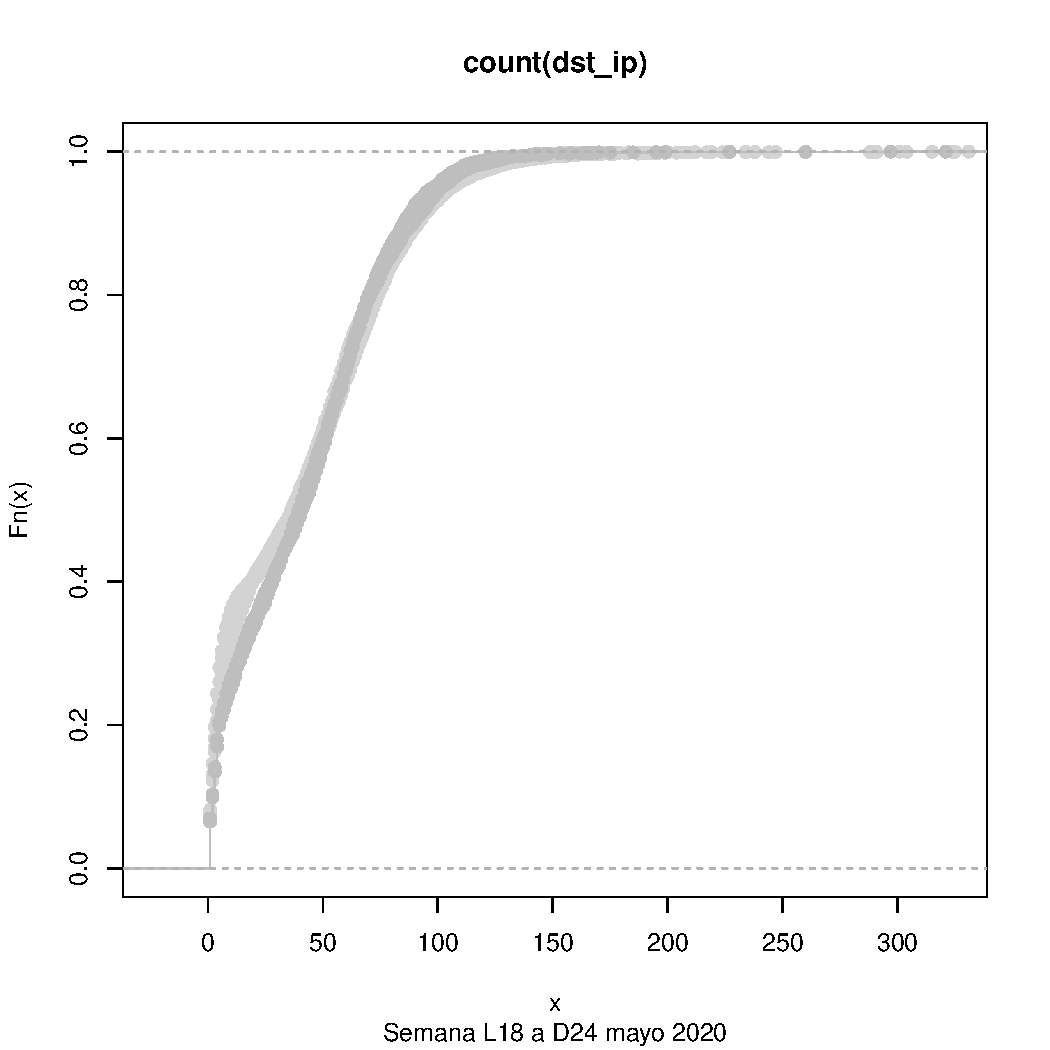
\includegraphics[width=0.3\textwidth]{contenido/fig/ecdf-count_dst_ip.pdf}
    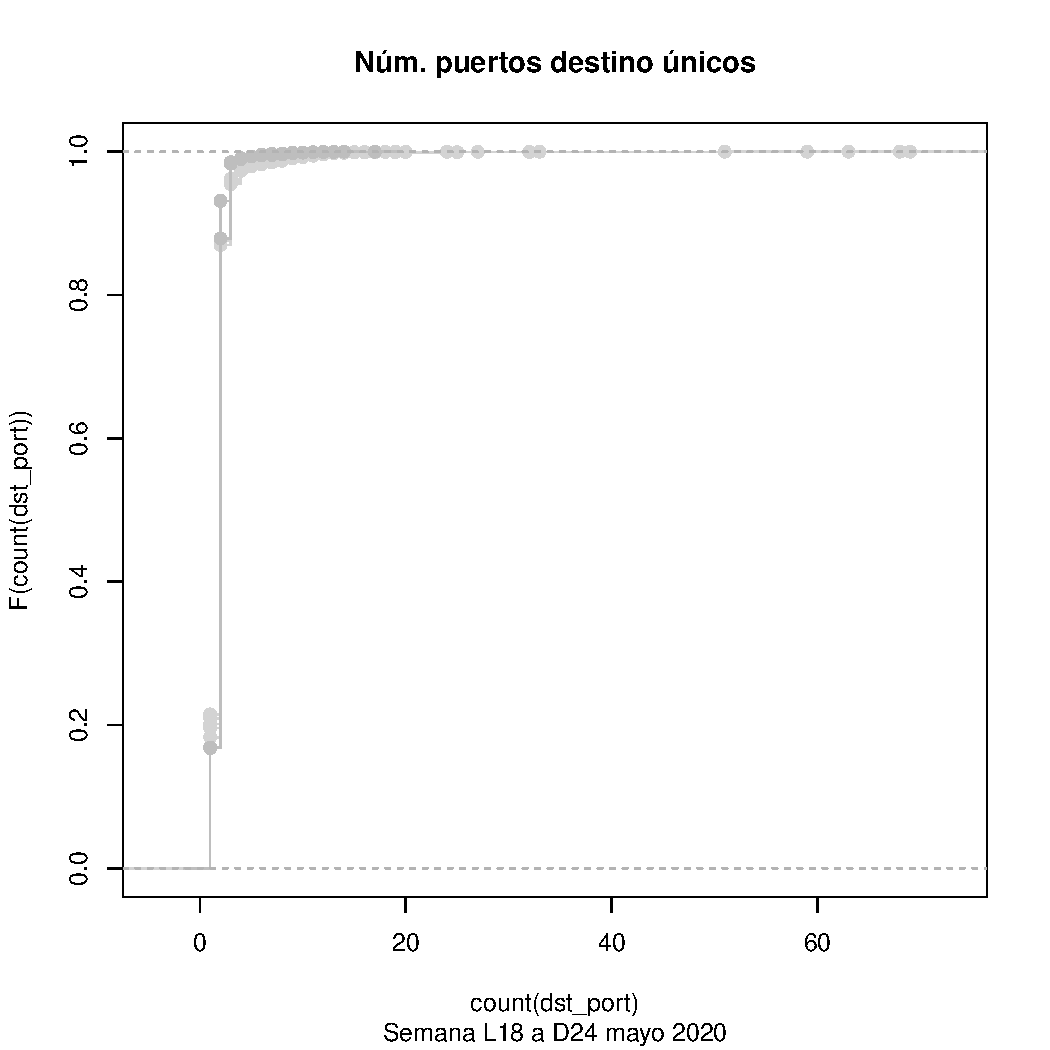
\includegraphics[width=0.3\textwidth]{contenido/fig/ecdf-count_dst_port.pdf}
    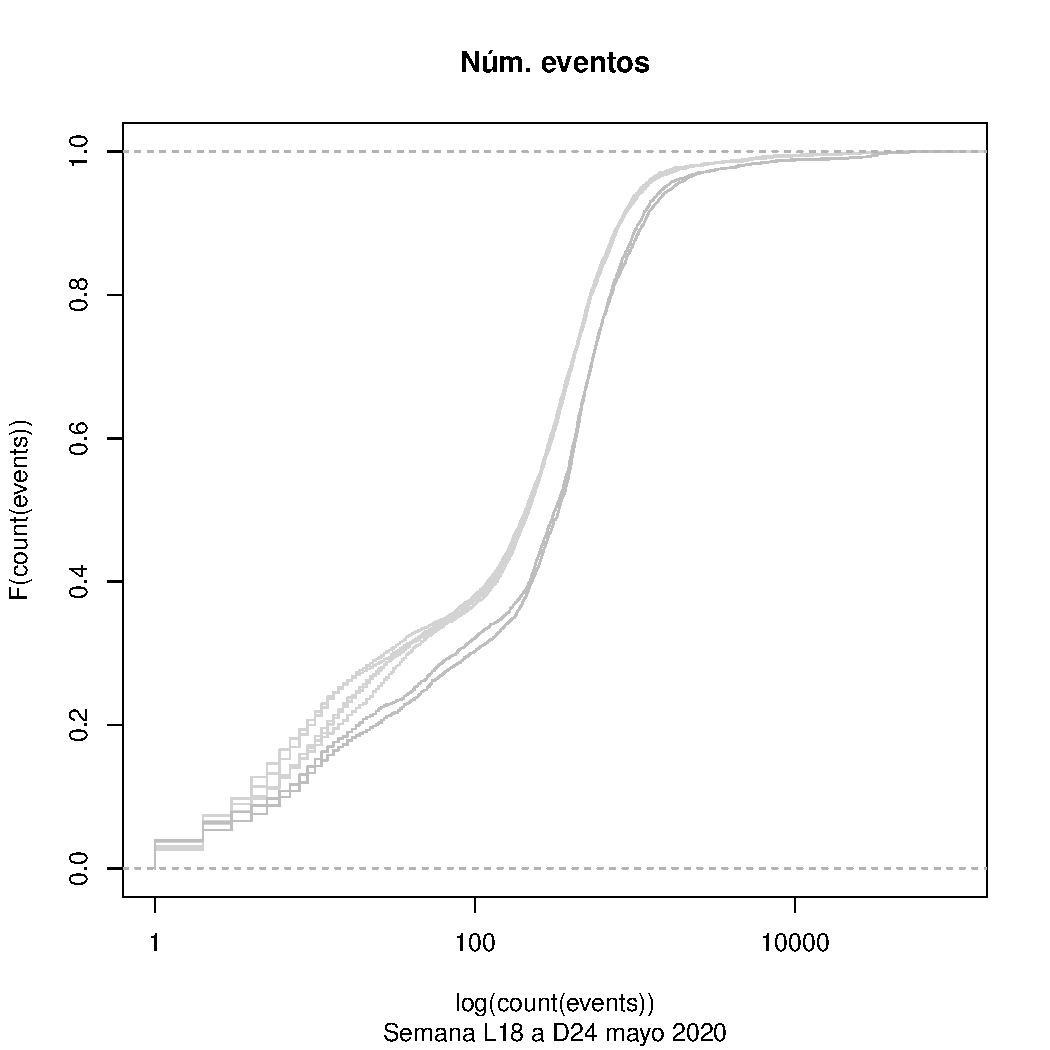
\includegraphics[width=0.3\textwidth]{contenido/fig/ecdf-count_events.pdf}
    %\subfigure[]{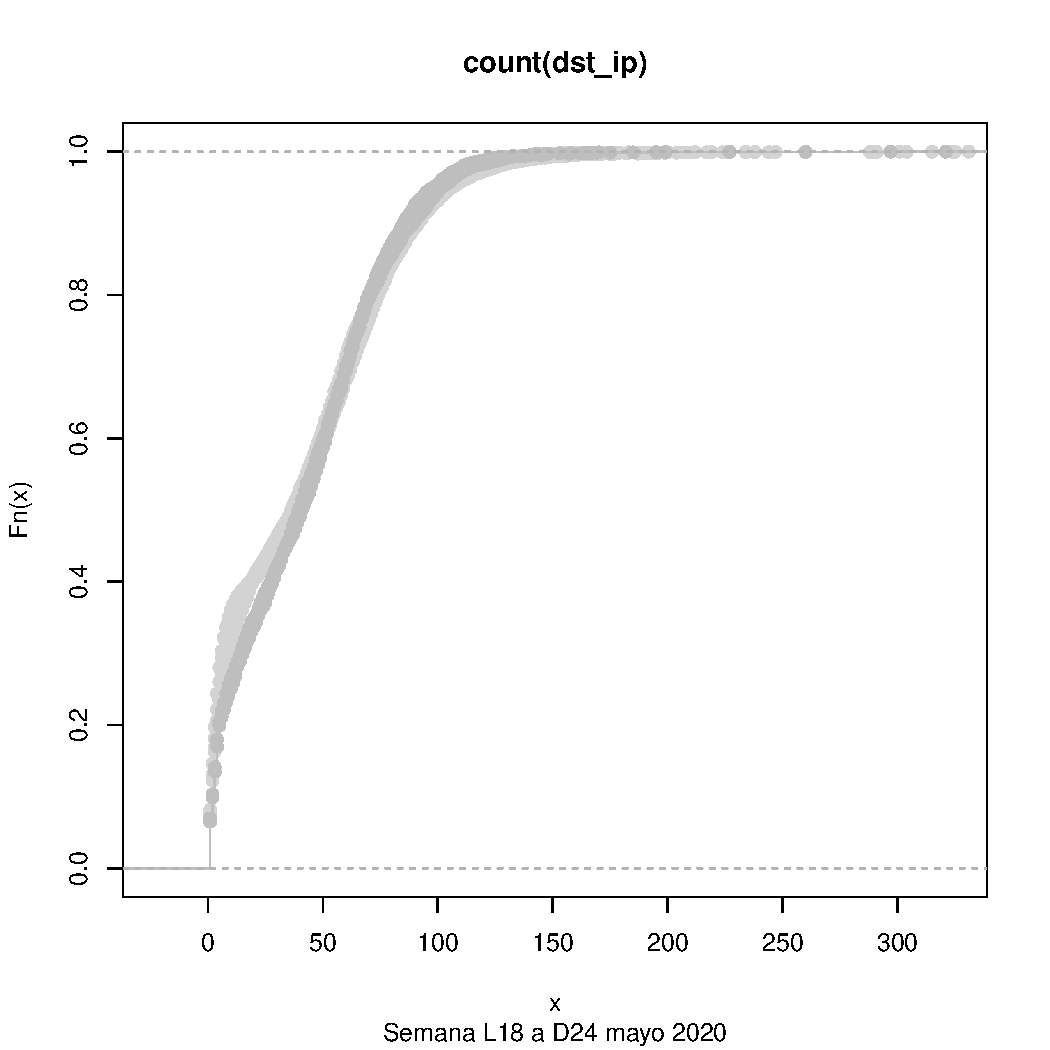
\includegraphics[width=0.3\textwidth]{contenido/fig/ecdf-count_dst_ip.pdf}}
    %\subfigure[]{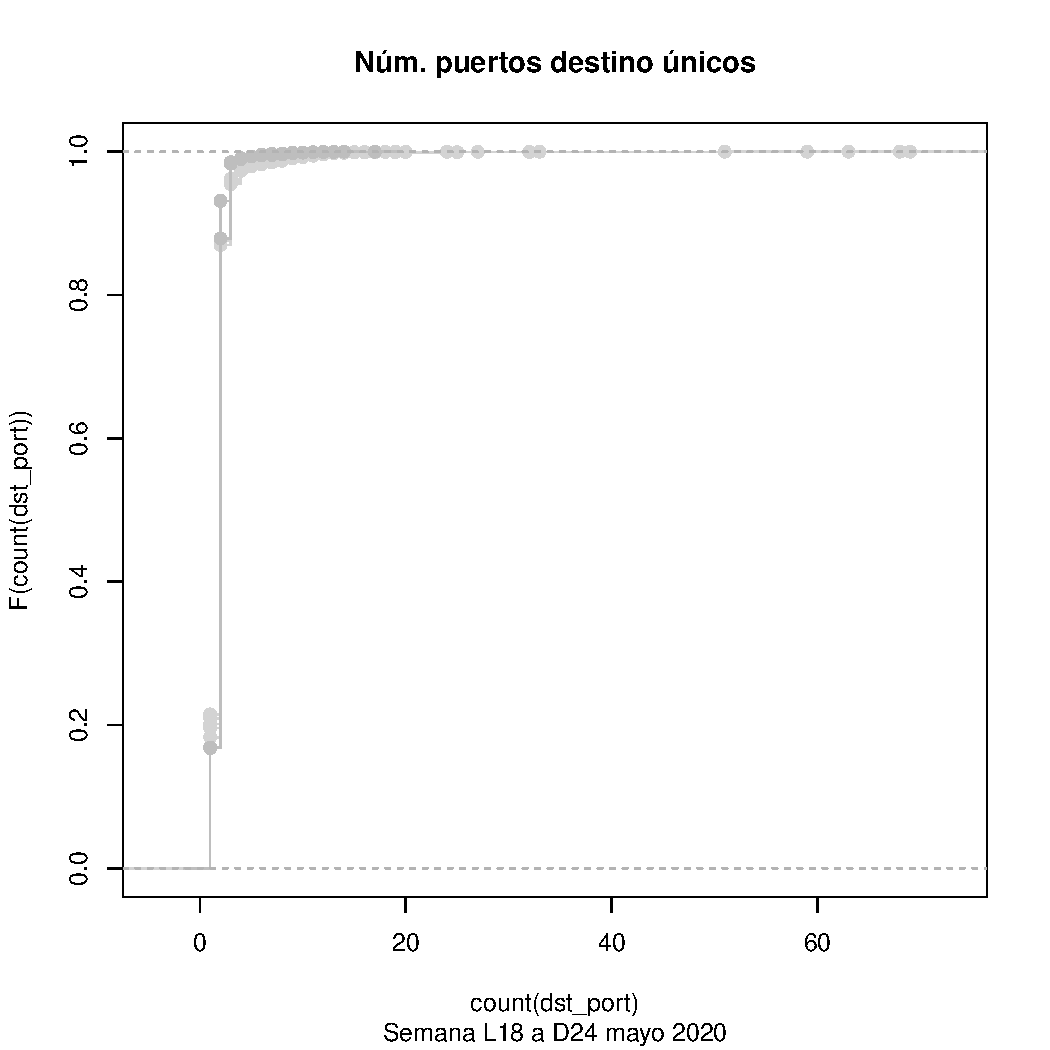
\includegraphics[width=0.3\textwidth]{contenido/fig/ecdf-count_dst_port.pdf}}
    %\subfigure[]{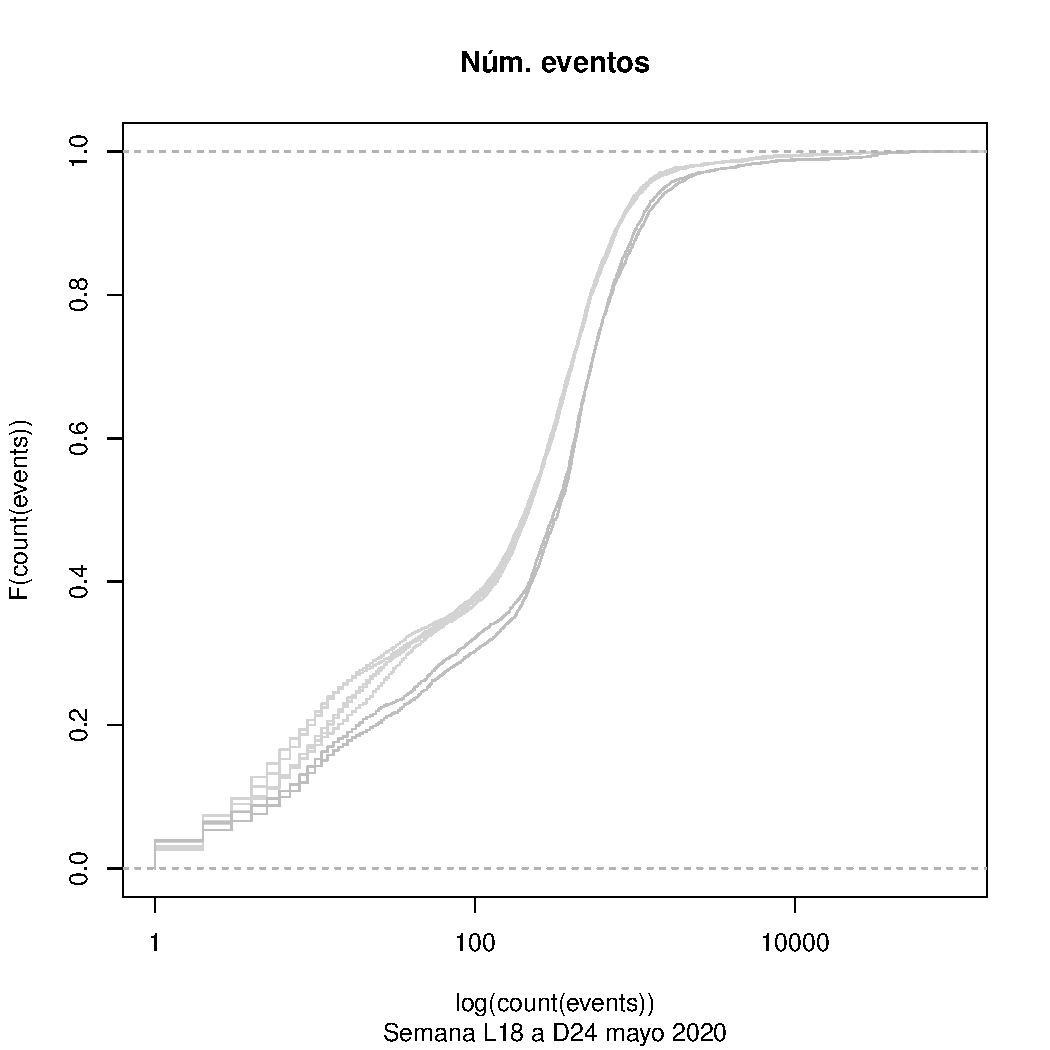
\includegraphics[width=0.3\textwidth]{contenido/fig/ecdf-count_events.pdf}}
    \caption{Funciones de distribución acumulada por número de IPs destino, puertos destino y eventos}
    \label{fig:ecdfcountdstip}
\end{figure}

La figura \ref{fig:ecdfcountdstip} muestra la función de distribución acumulada para varias características elegidas entre los datos disponibles.
Se han superpuesto las siete líneas de los días de la semana extraída, de forma que se evidencia la estabilidad de estas distribuciones a lo largo de los días.
Se representa cada variable sin normalizar, con lo que se obtiene una idea del rango de valores en el que se encuentra cada una.
Cuando se pase a computar los \emph{clusters}, se normalizarán para evitar que los atributos con escalas mayores dominen las distancias.

En el caso del número de eventos, se aprecia que es la distribución que más se acerca a una gaussiana, con una varianza un poco mayor en los días del fin de semana
(son los que quedan por debajo porque tienen más varianza y una media algo superior, coloreados con un gris algo más oscuro).
Pero, por lo general, las distribuciones que presenta el resto de características no son gaussianas y muestran asimetría positiva (los valores se concentran a la izquierda).

Por tanto, se espera que las colas de las distribuciones (es decir, los puntos con valores más altos) sean de más interés en el \emph{clustering}.
También se espera que los algoritmos sitúen a la gran mayoría de puntos dentro de unos pocos \emph{clusters} bastante densos.
Esto es una ventaja de cara al objetivo de detectar anomalías.

Como análisis preliminar al prototipado de métodos de \emph{clustering} mediante la herramienta BigML\footnote{\url{https://bigml.com/}},
se visualizaron varias parejas de variables sobre un gráfico de dispersión, con la finalidad de adquirir una idea de sus dimensiones y cómo se relacionaban.
Se aplicó también K-Means con varios valores de $k$, distinguiendo por colores los grupos formados, y se situaron los centroides en la gráfica (puntos rojos).
Así se empezó a entender qué divisiones podían establecerse y dónde podrían encontrarse los umbrales,
aunque de momento solo se estuvieran teniendo en cuenta subconjuntos reducidos de las características disponibles.

\begin{figure}[h]
    \centering
    \captionsetup{width=0.75\textwidth}
    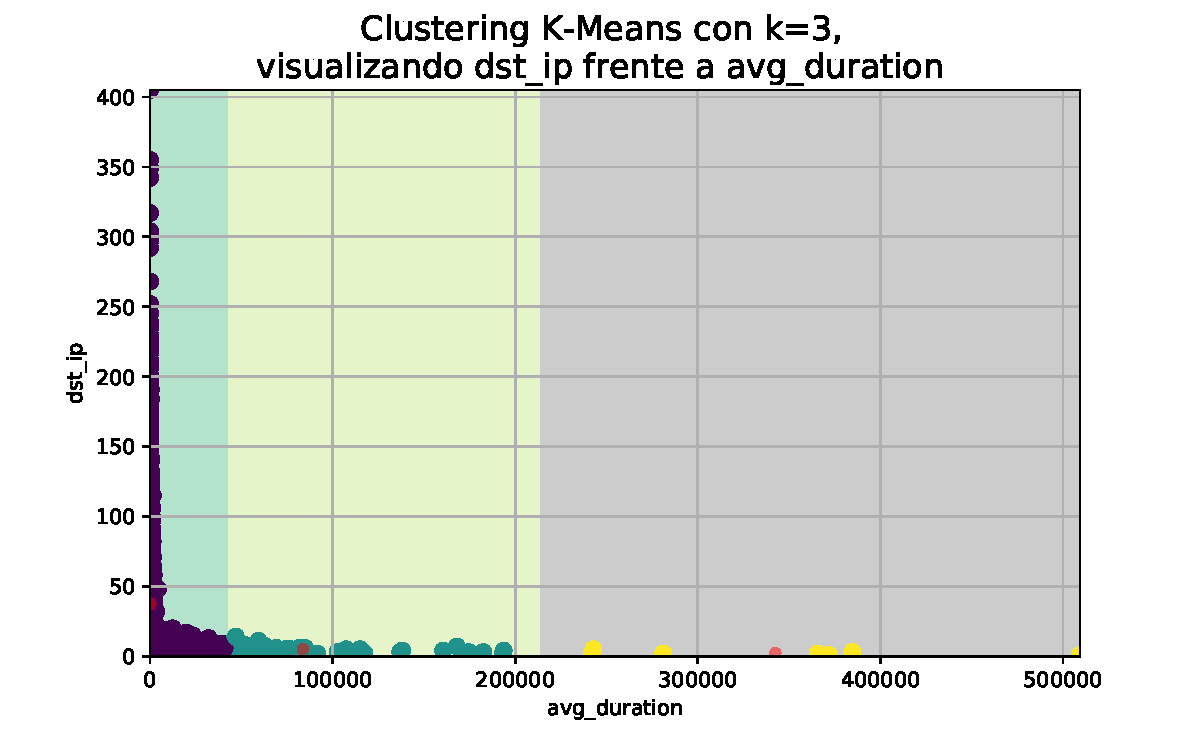
\includegraphics[width=0.9\textwidth]{contenido/fig/dispersion-k3-dst_ip-vs-avg_duration.pdf}
    \caption{Gráfica de dispersión: número de IPs destino únicas frente a duración media, con K-Means ($k=3$) y centroides (en rojo)}
    \label{fig:scatterdstipavgduration}
\end{figure}

\begin{figure}[h]
    \centering
    \captionsetup{width=0.75\textwidth}
    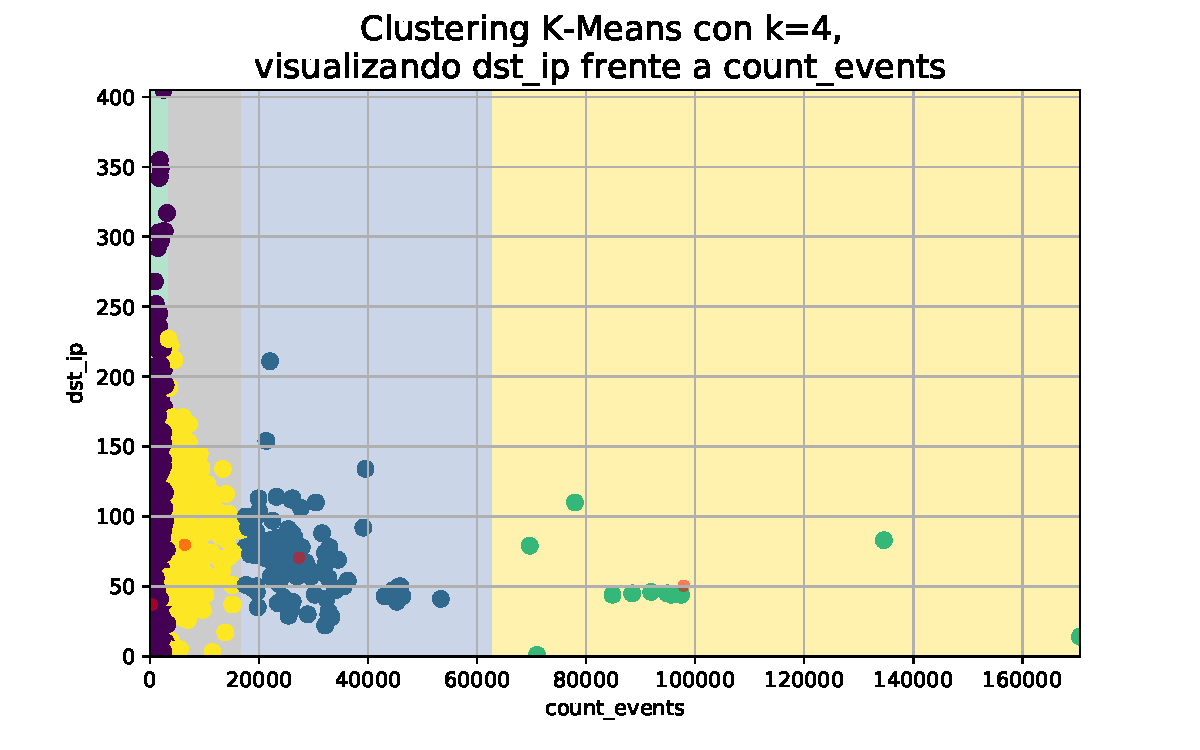
\includegraphics[width=0.9\textwidth]{contenido/fig/dispersion-k4-dst_ip-vs-count_events.pdf}
    \caption{Gráfica de dispersión: número de IPs destino únicas frente a número de eventos, con K-Means ($k=4$) y centroides (en rojo)}
    \label{fig:scatterdstipcountevents}
\end{figure}

Las figuras \ref{fig:scatterdstipavgduration} y \ref{fig:scatterdstipcountevents} son una muestra de estas pruebas.
En ellas, se aprecia cómo se reparten los puntos según los valores que toman en características como ``número de IPs destino únicas'', ``duración media'' o ``número de eventos'',
así como los \emph{clusters} formados en función del valor de $k$ elegido.
Se han elegido estas características porque presentan unos rangos muy distintos y los valores observados están distribuidos en varias zonas de dichos rangos,
por lo que se diferencia una serie de grupos que pueden corresponder a algunos de los comportamientos de equipos informáticos en los que estamos interesados.

En la sección \ref{sec:paramclustering} se ampliará cómo se buscaron los valores de $k$ con los que se trabajaría.

\section{Selección de características}\label{sec:selecciondecaracteristicas}

Como se apunta en ``Análisis de las características en tráfico de red para detección de anomalías'' \cite{Iglesias_2015},
la meta que tiene la selección de características en la detección de anomalías es
``eliminar características fuertemente correladas, redundantes e irrelevantes para mejorar la calidad de la detección''.
En este trabajo, los autores abordaron la selección de características de forma exhaustiva y rigurosa,
mediante métodos multi-fase implementados con envolvedores (\emph{wrappers}, que buscan el subconjunto de características con mejores resultados),
combinando filtrado y técnicas de regresión gradual.
Para nuestro caso, se ha optado por un procedimiento más sencillo, fundamentado en dos factores: la correlación entre características y la aportación de cada una al agrupamiento.

De acuerdo con la argumentación de \cite{Bohara_2016}, si las características de un conjunto están altamente correladas,
contendrán información redundante y provocarán un incremento innecesario de la complejidad del algoritmo.
Para evitar esta redundancia, en dichos conjuntos fuertemente correlados se seleccionará una única característica.
La correlación puede determinarse empleando el coeficiente de correlación de Pearson.
Se decide que dos características se tomarán como fuertemente correladas si su coeficiente de correlación es mayor de 0,99.
Ya que se tiene un \emph{dataset} de tamaño bastante grande y el rango de valores de las características está acotado,
se espera que el coeficiente de correlación de Pearson proporcione una estimación de la correlación suficientemente precisa.

El otro aspecto a considerar es la contribución de cada característica en la fase de \emph{clustering}.
Si, al analizar el vector de los pesos relativos que tiene cada característica sobre cada uno de los \emph{clusters},
se aprecia que ciertas características tienen un papel poco activo en la clasificación,
se simplificará el set de características eliminando aquellas que aportan débilmente al algoritmo.

Es importante distinguir la sutil diferencia entre selección de características y extracción de características.
Ambos son métodos para reducir la dimensionalidad, pero el proceso que siguen es distinto.
La selección de características descarta características irrelevantes o redundantes para los procesos posteriores de representación y clasificación de datos.
En cambio, la extracción de características consiste en proyectar el \emph{dataset} original en un nuevo espacio vectorial
donde se minimice la dependencia lineal entre características, reduciendo por tanto el número de variables necesarias.
Aunque estas técnicas (por ejemplo, el análisis de componentes principales o PCA) permiten ponderar la importancia de las características y por tanto seleccionarlas,
debe destacarse que solo consideran relaciones lineales entre variables (ignorando cualquier otro tipo de interacción entre ellas).
Por eso se puede afirmar que no es un método ideal para seleccionar características, si bien es cierto
que pueden combinarse selección y extracción de características, eliminando características irrelevantes primero y proyectándolas en espacios optimizados después.

También se valora la observación de \cite{Guyon_2003} cuando dice que ``el objetivo de la selección de variables es triple: mejorar el rendimiento de los predictores, posibilitar predictores más rápidos y eficientes en coste, y permitir una mejor comprensión del proceso subyacente que ha generado los datos''.
La selección de características aquí expuesta busca cumplir con estas tres finalidades.

Tras hacer tests de correlación entre todas las variables, no se ha encontrado ninguna pareja de variables con tanta correlación como para poder suprimir una de ellas.
Sin embargo, sí se ha comprobado que puede reducirse el número de variables (y con ello el coste y complejidad del \emph{clustering}) quedándose solo con las de mayor peso.
Tras analizar la importancia relativa de cada una en los modelos generados tras el clustering (se adjuntan cifras concretas en los apéndices),
se ha repetido el último ensayo (indicado en la subsección \ref{subsec:ensayoD}) manteniendo solo las 6 características más influyentes: ``dst\_ip'', ``proto'', ``src\_port'', ``max\_prio'' y ``count\_events''.
El resultado ha sido que se lograban los mismos \emph{clusters} y el mismo número de instancias en el \emph{cluster} de anomalías, con un considerable decremento del tiempo de computación.

Contrariamente a lo que se esperaba, esto indica que las variables temporales no han sido tan decisivas como se creía que serían.

\section{Parametrización del algoritmo de clustering}\label{sec:paramclustering}

Elegir un número $k$ de \emph{clusters} óptimo es crucial para obtener una clasificación útil.
Si el número de \emph{clusters} es insuficiente, las agrupaciones contendrán datos muy heterogéneos.
Por el contrario, cuando el valor $k$ es excesivo, se agruparán erróneamente datos que son muy similares unos a otros.

Aunque no existe un único criterio que seleccione objetivamente el valor $k$ adecuado para cualquier caso, sí se conocen varios métodos que ayudan en esta tarea.
Probablemente uno de los más extendidos sea el método del codo o \emph{elbow method}.

Una de las medidas que se suelen utilizar para comparar resultados entre varios valores de $k$ es la suma de cuadrados dentro de cada grupo (\emph{within-cluster sums of squares}, abreviado como WCSS).
Este concepto a veces también se conoce como inercia, y es una medida de variación o desviación con respecto a la media, en este caso representada por el centroide.
La técnica de selección de $k$ por el método del codo consiste en representar en una gráfica lineal la WCSS respecto del número de \emph{clusters}.
El punto para el cual se observe un cambio brusco en la evolución de la inercia indicará el valor óptimo de $k$.

La efectividad de este método está basada en que el algoritmo K-Means se fundamenta en el paradigma del análisis de la varianza (\emph{analysis of variance} o ANOVA).
Como la suma total de desviaciones al cuadrado respecto de los centroides es constante y está compuesta de la suma de cuadrados de las desviaciones inter-grupales más la de las desviaciones intra-grupales:

\begin{eqnarray*}
    & TSS = WCSS + BCSS \\
    & SS_{Total} = SS_{Within-cluster} + SS_{Between-clusters}
\end{eqnarray*}

Si se minimiza la suma de cuadrados dentro de cada \emph{cluster} (WCSS), se maximiza la distancia entre \emph{clusters}.
De esta forma, se logrará una separación en grupos adecuada, siempre que esta suma de cuadrados WCSS no sea tanta como para asociar puntos cercanos pero de distintas categorías.

En la figura \ref{fig:codo} se muestra la gráfica lineal de WCSS respecto de $k$ que se ha explicado, calculada para varios subconjuntos de características.
Se puede observar que el valor de $k$ que este método daría como óptimo es distinto según las variables consideradas, y no es inequívocamente claro.

\begin{figure}[h!]
    \centering
    \captionsetup{width=0.75\textwidth}
    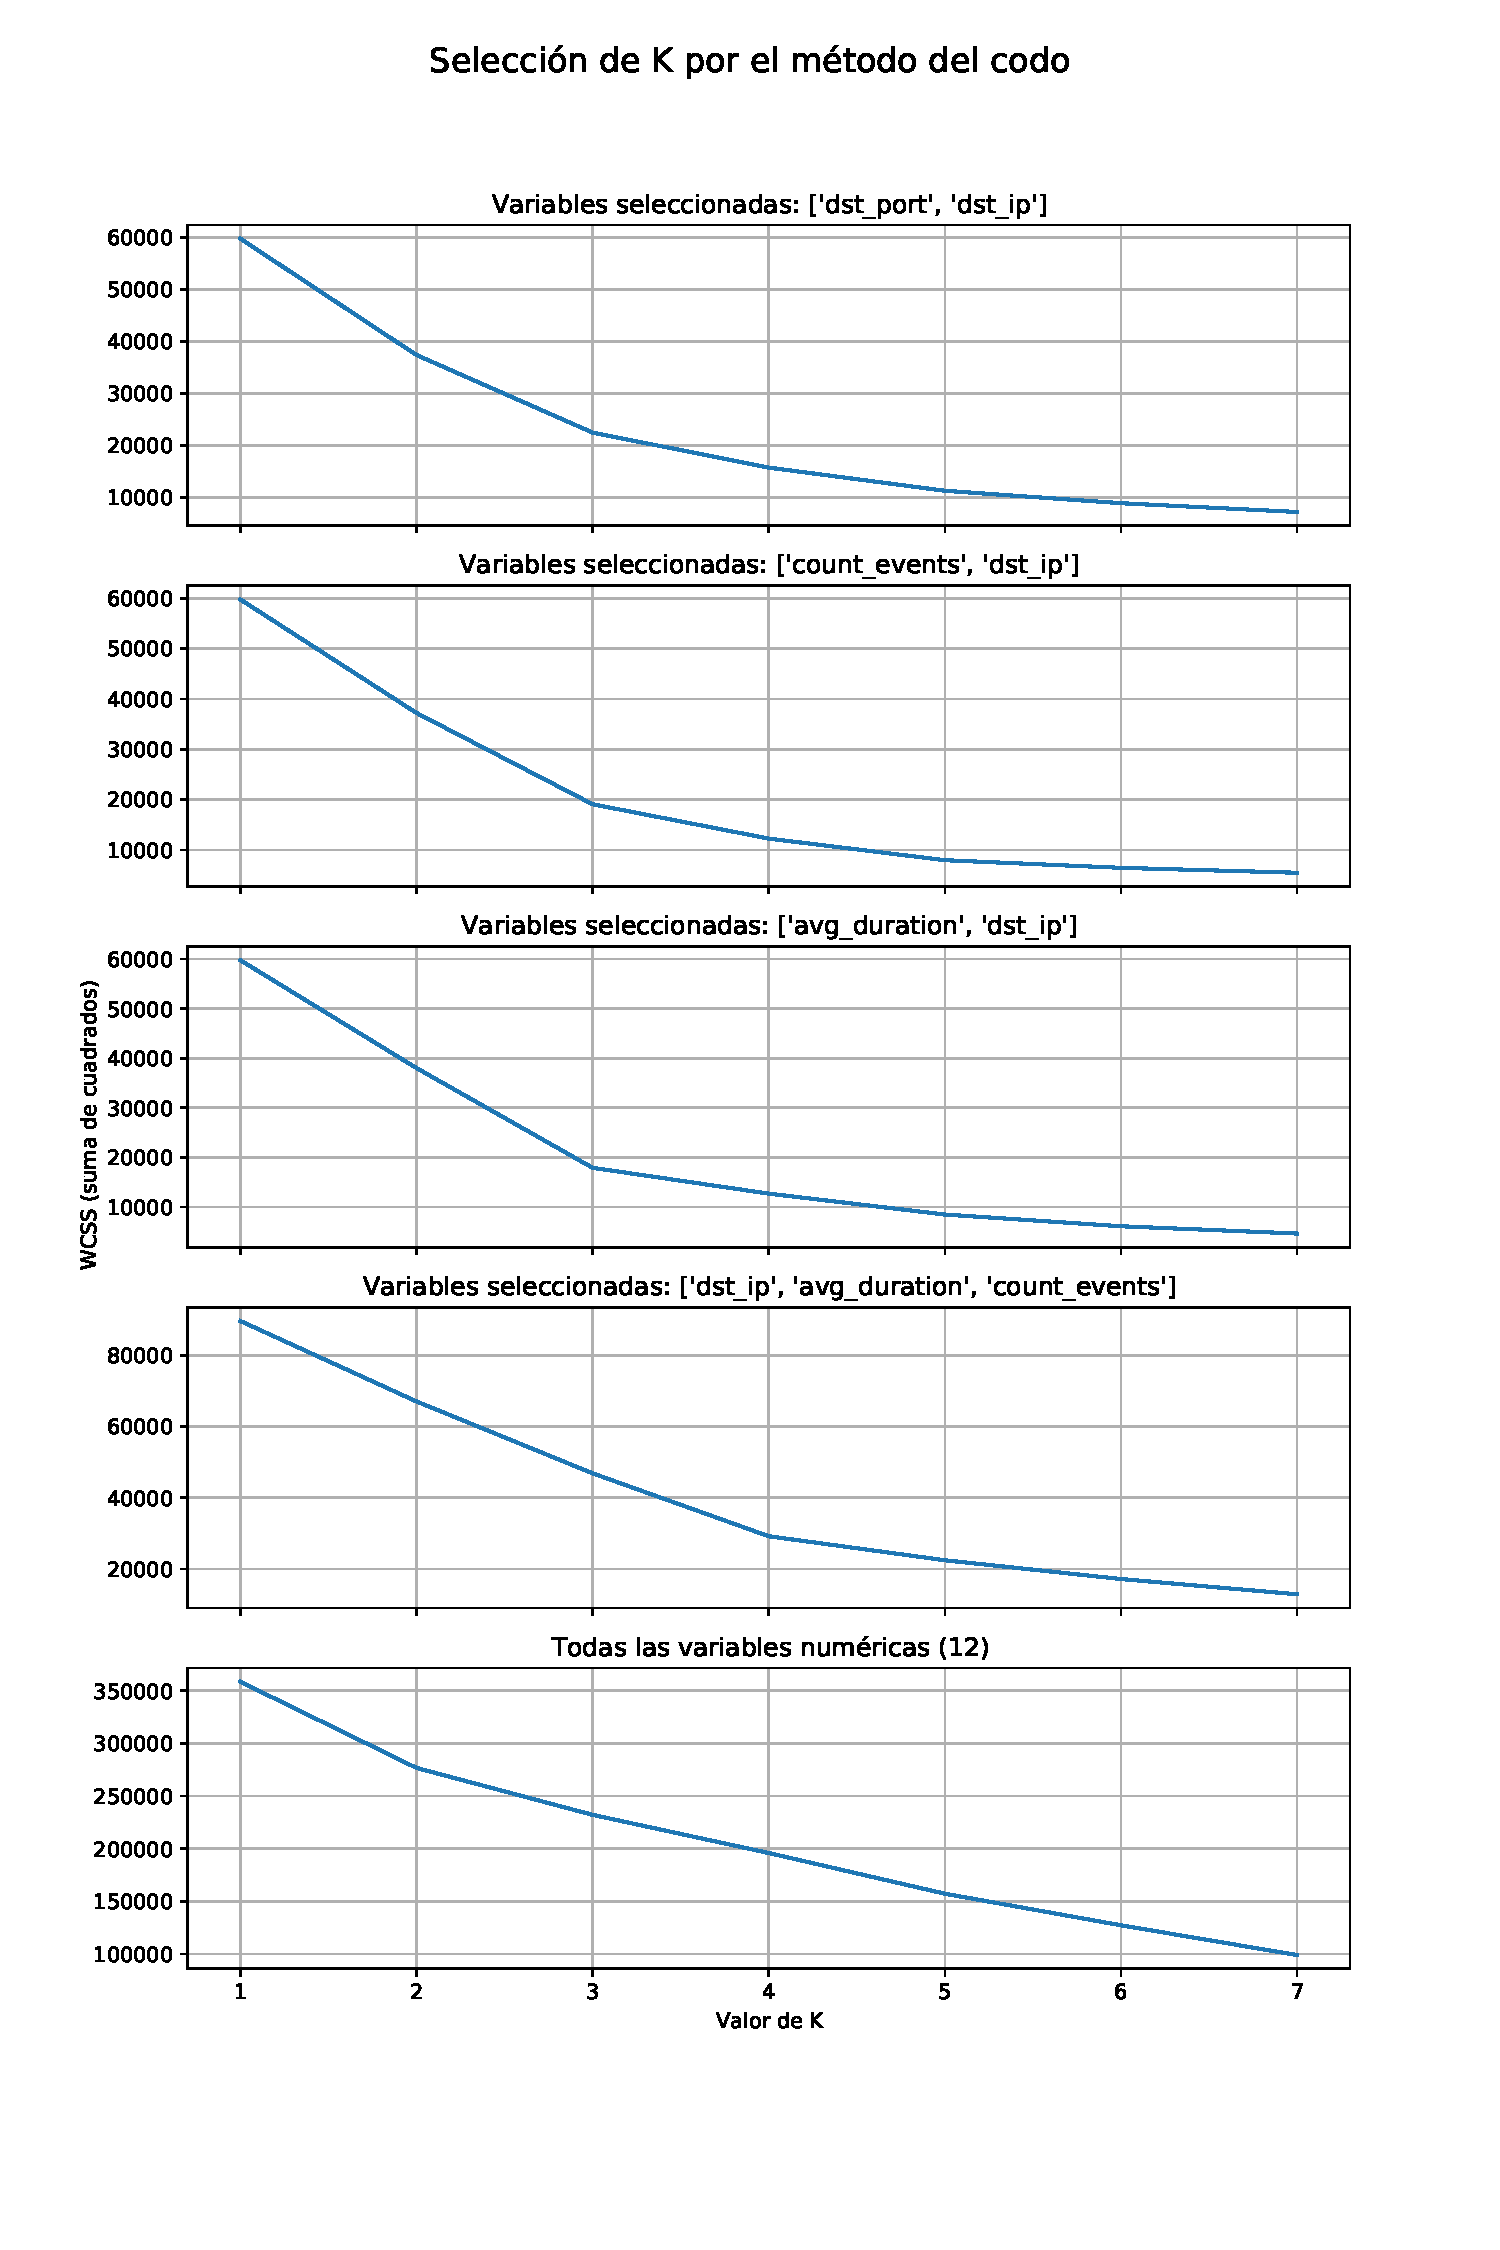
\includegraphics[width=0.9\textwidth]{contenido/fig/codo.pdf}
    \caption{Gráficas de suma de cuadrados frente a valores de $k$ en varias combinaciones seleccionadas de características}
    \label{fig:codo}
\end{figure}

Tras las pruebas experimentales que se describen en la siguiente sección, se concluyó que el valor de $k$ que arrojó mejores resultados empíricamente fue $k=5$.

\section{Evaluación experimental}\label{sec:evaluacionexperimental}

Con la máxima de permitir un prototipado rápido y poder comparar los resultados de varias pruebas,
se optó por emplear la herramienta online BigML para aplicar K-Means en los ensayos que se procede a explicar.

\subsection{Ensayo A: K-Means con k=5, sin características temporales}\label{subsec:ensayoA}

Como se adelantaba en la sección \ref{sec:preprocesado}, en las primeras pruebas no se incluyeron las marcas de tiempo.
Se usaron las características anotadas como ``dst\_ip'', ``proto'', ``src\_port'', ``dst\_port'', ``anom\_level'', ``max\_prio'', ``count\_events'' y ``avg\_duration'',
junto con ``src\_ip'' como característica identificativa.
Después se advirtió que usar únicamente la media para resumir la información sobre la duración de las sesiones de un equipo durante un día parecía impreciso,
así que se incluyó la característica ``stdev\_duration''.

Inicialmente se eligieron valores $k=3$ y $k=4$, pero las divisiones obtenidas resultaron de poca utilidad desde el punto de vista de la caracterización de comportamientos.
Los \emph{clusters} principales agrupaban demasiadas instancias sin un criterio fácil de deducir, y el \emph{cluster} minoritario contenía únicamente algunas instancias con valores extremos.

Fijando el valor de $k=5$ se mejoró sensiblemente la interpretabilidad de los \emph{clusters} formados,
porque sus centroides pudieron asociarse a patrones de comportamiento más claros.

Las categorías identificadas en los \emph{clusters} formados durante este ensayo fueron:
\begin{enumerate}
    \item Comportamiento normal, muchas conexiones (54,34 \% de las instancias)
    \item Comportamiento normal, pocas conexiones (30,96 \%)
    \item Sesiones UDP (14,12 \%)
    \item Nivel de anomalía alto (0,45 \%)
    \item Conexiones largas (0,14 \%)
\end{enumerate}

En el apéndice \ref{app:ensayoA} se pueden consultar los detalles de la salida que produjo la aplicación de K-Means con $k=5$ en estas condiciones.
Se adjuntan datos de interés como los valores de las 10 características con los que se definía el centroide de cada \emph{cluster}.
Se incluyen también los modelos de cada \emph{cluster} que ofrece BigML, definidos mediante algunas reglas de clasificación.
Si se revisan las reglas generadas automáticamente para este ensayo y otros, se encontrará que a veces consideran características que no tienen mucho sentido.
Por eso las reglas pueden ser útiles para establecer ciertos umbrales, pero no deben seguirse a ciegas, independientemente de sus niveles de confianza y soporte.

Además, en el apéndice se listan las características que han contribuido a la formación de cada \emph{cluster} ordenadas por influencia.
Esta última información resulta muy interesante a la hora de comprender y optimizar la manera en la que se ha alcanzado esta clasificación no supervisada.
Servirá también de realimentacion para mejorar la selección de características comentada en la sección \ref{sec:selecciondecaracteristicas}.

En unas pruebas adicionales, se intentó incluir una dimensión temporal mediante la característica ``active\_hours\_vector''.
Esta contenía un vector con 24 valores que representaban el número de sesiones que tenía una IP origen en cada hora del día.
Se trató primero como una característica categórica (interpretando estos valores como items en vez de valores numéricos) y luego como 24 características numéricas independientes,
pero no se tuvieron buenos resultados.
Por eso se replanteó el preprocesado de estos datos temporales y finalmente se fijó el conjunto de características de la tabla \ref{tab:metricas}.

\subsection{Ensayo B: G-Means determina k=3}\label{subsec:ensayoB}

Con el \emph{dataset} final, se decidió probar el algoritmo G-means (\emph{Gaussian-means}) que ofrece BigML.
Este algoritmo descubre el número $k$ de \emph{clusters} automáticamente, usando un test estadístico para decidir si dividir un centroide en dos.
El algoritmo procede jerárquicamente, fijándose en un subconjunto de datos, y en cada iteración testea la hipótesis de que el subconjunto sigue una distribución gaussiana.
Si no la sigue, divide el \emph{cluster}.

Este algoritmo puede ser útil si no se tiene una estimación de cuál puede ser el valor de $k$ adecuado, presuponiendo unos datos de distribución normal.
Sin embargo, se comprobó que el algoritmo no era apropiado para este caso, ya que los 3 \emph{clusters} resultantes no eran significativos para la aplicación en cuestión.
Además, era de esperar que no funcionara bien con estos datos, porque en la sección \ref{sec:analisisdedatos} se había visto que la distribución de la mayoría de las variables no coincidía con una gaussiana.

Se adjuntan los resultados de esta prueba en el apéndice \ref{app:ensayoB}, por constatar lo que se ha descrito aquí.

\subsection{Ensayo C: K-Means con k=5, fracciones temporales con agrupación semanal}\label{subsec:ensayoC}

Se pasó entonces al \emph{clustering} usando K-Means con $k=5$ sobre el \emph{dataset} final.
En primer lugar se agrupó toda la información en un solo vector de características de la sesión, sin separar por días.
El informe completo del resultado está en el apéndice \ref{app:ensayoC},
pero puede resumirse con que se lograron unos \emph{clusters} ya bastante similares a los que se ampliarán en la próxima subsección y en el capítulo \ref{chap:resultados} de resultados.
Dichos resultados son los que se tomaron como los mejores.

No obstante, el \emph{cluster} de anomalías se componía de solo 3 instancias que,
según revelaba el resumen del modelo de este \emph{cluster}, se habían agrupado únicamente por sus valores altos en la característica ``duración media''.
Se consideró que la condensación de información en el preprocesado (los datos de toda la semana se expresaban con un único punto) estaba siendo demasiada.

Además, el ratio de sumas de cuadrados ($SS_{Between-clusters} / SS_{Total}$) era de 0.3358,
un indicador de que sería conveniente mejorar las propiedades de cohesión interna y separación interna del \emph{clustering}.
En términos estadísticos, esto se consigue incrementando la suma de cuadrados inter-grupales y reduciendo la suma de cuadrados intra-grupales,
hecho que se dio al hacer una agrupación diaria en el preprocesado.

\subsection{Ensayo D: K-Means con k=5, fracciones temporales con agrupación diaria}\label{subsec:ensayoD}

En el último ensayo se aplicó K-Means con $k=5$ por separado a los 7 \emph{datasets} que se tenían cuando se hizo agrupación diaria sobre los datos de una semana.
Los resultados (completos en el apéndice \ref{app:ensayoD}) eran más claros y útiles que los de ensayos anteriores.

Las categorías finales en las que se clasificó la actividad de los equipos de la red en cada día fueron:
\begin{enumerate}
    \item Comportamiento normal, muchas conexiones (de media 54,07 \% de las instancias)
    \item Comportamiento normal, pocas conexiones (de media 30,34 \%)
    \item Sesiones UDP (de media 8,05 \%)
    \item Conexiones largas o muchas IPs destino (de media 7,42 \%)
    \item Anomalías: muchos eventos y conexiones (0,30 \%)
\end{enumerate}

En el siguiente capítulo se entra de lleno a explicar los resultados obtenidos en este ensayo final.
